% Created by tikzDevice version 0.12.6 on 2024-08-15 14:40:36
% !TEX encoding = UTF-8 Unicode
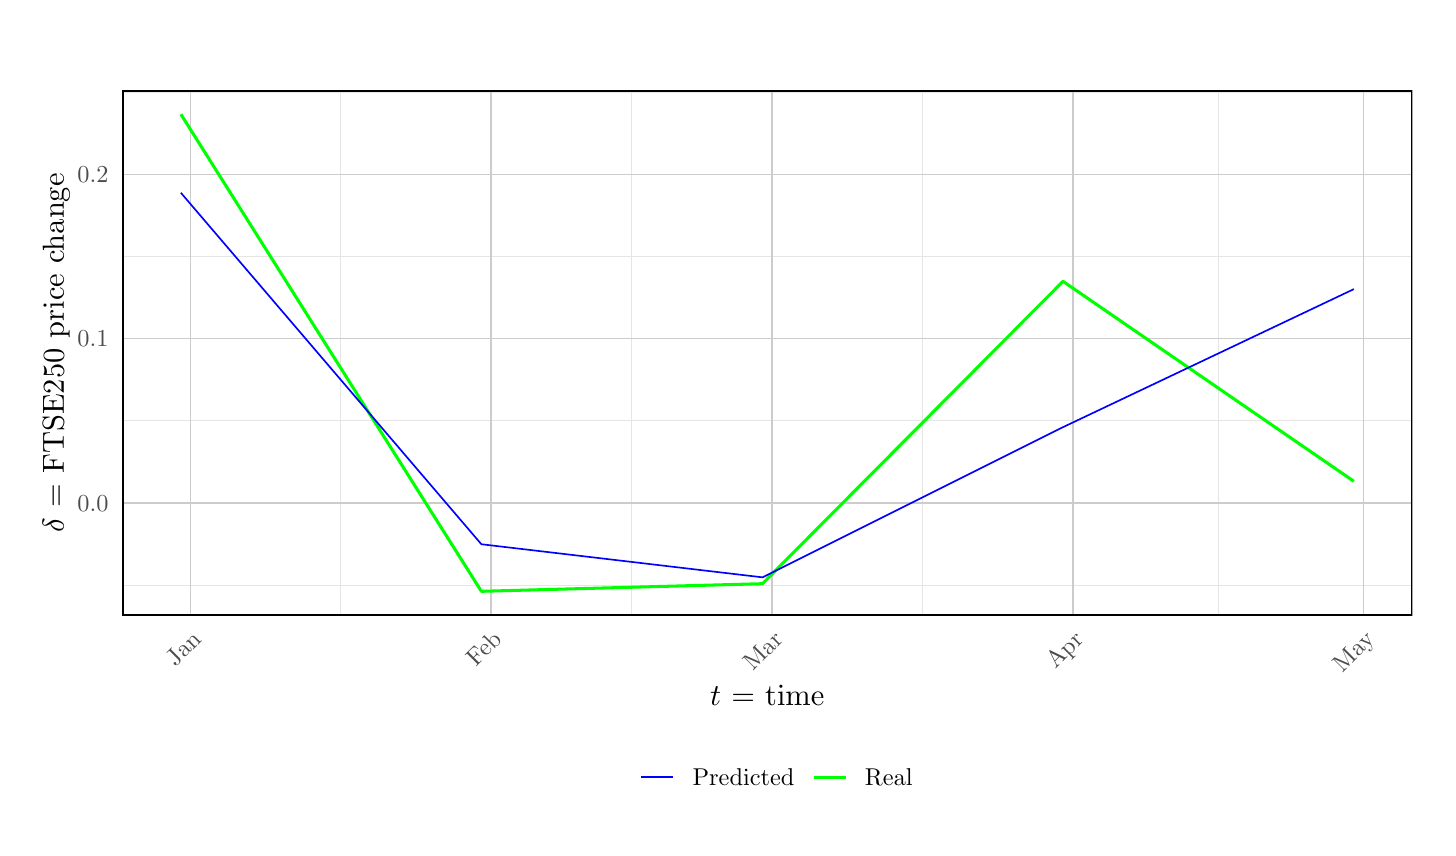
\begin{tikzpicture}[x=1pt,y=1pt]
\definecolor{fillColor}{RGB}{255,255,255}
\path[use as bounding box,fill=fillColor,fill opacity=0.00] (0,0) rectangle (505.89,289.08);
\begin{scope}
\path[clip] ( 34.16, 76.79) rectangle (500.39,266.42);
\definecolor{drawColor}{gray}{0.90}

\path[draw=drawColor,line width= 0.3pt,line join=round] ( 34.16, 87.71) --
	(500.39, 87.71);

\path[draw=drawColor,line width= 0.3pt,line join=round] ( 34.16,147.06) --
	(500.39,147.06);

\path[draw=drawColor,line width= 0.3pt,line join=round] ( 34.16,206.41) --
	(500.39,206.41);

\path[draw=drawColor,line width= 0.3pt,line join=round] ( 34.16,265.76) --
	(500.39,265.76);

\path[draw=drawColor,line width= 0.3pt,line join=round] (113.15, 76.79) --
	(113.15,266.42);

\path[draw=drawColor,line width= 0.3pt,line join=round] (218.23, 76.79) --
	(218.23,266.42);

\path[draw=drawColor,line width= 0.3pt,line join=round] (323.32, 76.79) --
	(323.32,266.42);

\path[draw=drawColor,line width= 0.3pt,line join=round] (430.16, 76.79) --
	(430.16,266.42);
\definecolor{drawColor}{gray}{0.80}

\path[draw=drawColor,line width= 0.6pt,line join=round] ( 34.16,117.38) --
	(500.39,117.38);

\path[draw=drawColor,line width= 0.6pt,line join=round] ( 34.16,176.73) --
	(500.39,176.73);

\path[draw=drawColor,line width= 0.6pt,line join=round] ( 34.16,236.08) --
	(500.39,236.08);

\path[draw=drawColor,line width= 0.6pt,line join=round] ( 58.85, 76.79) --
	( 58.85,266.42);

\path[draw=drawColor,line width= 0.6pt,line join=round] (167.44, 76.79) --
	(167.44,266.42);

\path[draw=drawColor,line width= 0.6pt,line join=round] (269.02, 76.79) --
	(269.02,266.42);

\path[draw=drawColor,line width= 0.6pt,line join=round] (377.61, 76.79) --
	(377.61,266.42);

\path[draw=drawColor,line width= 0.6pt,line join=round] (482.70, 76.79) --
	(482.70,266.42);
\definecolor{drawColor}{RGB}{0,255,0}

\path[draw=drawColor,line width= 1.1pt,line join=round] ( 55.35,257.80) --
	(163.94, 85.41) --
	(265.52, 88.16) --
	(374.11,197.41) --
	(479.20,125.17);
\definecolor{drawColor}{RGB}{0,0,255}

\path[draw=drawColor,line width= 0.6pt,line join=round] ( 55.35,229.43) --
	(163.94,102.42) --
	(265.52, 90.46) --
	(374.11,144.72) --
	(479.20,194.60);
\definecolor{drawColor}{RGB}{0,0,0}

\path[draw=drawColor,line width= 1.1pt,line join=round,line cap=round] ( 34.16, 76.79) rectangle (500.39,266.42);
\end{scope}
\begin{scope}
\path[clip] (  0.00,  0.00) rectangle (505.89,289.08);
\definecolor{drawColor}{gray}{0.30}

\node[text=drawColor,anchor=base east,inner sep=0pt, outer sep=0pt, scale=  0.88] at ( 29.21,114.35) {0.0};

\node[text=drawColor,anchor=base east,inner sep=0pt, outer sep=0pt, scale=  0.88] at ( 29.21,173.70) {0.1};

\node[text=drawColor,anchor=base east,inner sep=0pt, outer sep=0pt, scale=  0.88] at ( 29.21,233.05) {0.2};
\end{scope}
\begin{scope}
\path[clip] (  0.00,  0.00) rectangle (505.89,289.08);
\definecolor{drawColor}{gray}{0.30}

\node[text=drawColor,rotate= 45.00,anchor=base east,inner sep=0pt, outer sep=0pt, scale=  0.88] at ( 63.14, 67.55) {Jan};

\node[text=drawColor,rotate= 45.00,anchor=base east,inner sep=0pt, outer sep=0pt, scale=  0.88] at (171.73, 67.55) {Feb};

\node[text=drawColor,rotate= 45.00,anchor=base east,inner sep=0pt, outer sep=0pt, scale=  0.88] at (273.31, 67.55) {Mar};

\node[text=drawColor,rotate= 45.00,anchor=base east,inner sep=0pt, outer sep=0pt, scale=  0.88] at (381.90, 67.55) {Apr};

\node[text=drawColor,rotate= 45.00,anchor=base east,inner sep=0pt, outer sep=0pt, scale=  0.88] at (486.99, 67.55) {May};
\end{scope}
\begin{scope}
\path[clip] (  0.00,  0.00) rectangle (505.89,289.08);
\definecolor{drawColor}{RGB}{0,0,0}

\node[text=drawColor,anchor=base,inner sep=0pt, outer sep=0pt, scale=  1.10] at (267.27, 44.09) {$t$ = time};
\end{scope}
\begin{scope}
\path[clip] (  0.00,  0.00) rectangle (505.89,289.08);
\definecolor{drawColor}{RGB}{0,0,0}

\node[text=drawColor,rotate= 90.00,anchor=base,inner sep=0pt, outer sep=0pt, scale=  1.10] at ( 13.08,171.61) {$\delta$ = FTSE250 price change};
\end{scope}
\begin{scope}
\path[clip] (  0.00,  0.00) rectangle (505.89,289.08);
\definecolor{drawColor}{RGB}{0,0,255}

\path[draw=drawColor,line width= 0.6pt,line join=round] (221.75, 18.23) -- (233.31, 18.23);
\end{scope}
\begin{scope}
\path[clip] (  0.00,  0.00) rectangle (505.89,289.08);
\definecolor{drawColor}{RGB}{0,255,0}

\path[draw=drawColor,line width= 1.1pt,line join=round] (284.01, 18.23) -- (295.57, 18.23);
\end{scope}
\begin{scope}
\path[clip] (  0.00,  0.00) rectangle (505.89,289.08);
\definecolor{drawColor}{RGB}{0,0,0}

\node[text=drawColor,anchor=base west,inner sep=0pt, outer sep=0pt, scale=  0.88] at (240.26, 15.20) {Predicted};
\end{scope}
\begin{scope}
\path[clip] (  0.00,  0.00) rectangle (505.89,289.08);
\definecolor{drawColor}{RGB}{0,0,0}

\node[text=drawColor,anchor=base west,inner sep=0pt, outer sep=0pt, scale=  0.88] at (302.51, 15.20) {Real};
\end{scope}
\end{tikzpicture}
